\chapter{Appendix}

\section{Electronic Appendix}

To access all material relevant to this thesis, please refer to the respective GitLab repository which is available under: \url{https://gitlab.lrz.de/statistics/winter22/ma_schulzvanheyden}

It contains the following:
\begin{itemize}
    \item All of the data used.
    \item The embeddings from the semantic search methods.
    \item The code that is necessary to reproduce the analysis of this thesis with additional instructional clues on how to utilize it.
    \item A folder with the LaTeX project.
\end{itemize}

\newpage

\section{F1 Score Results}\label{f1}

\begin{figure}[h]
\centering
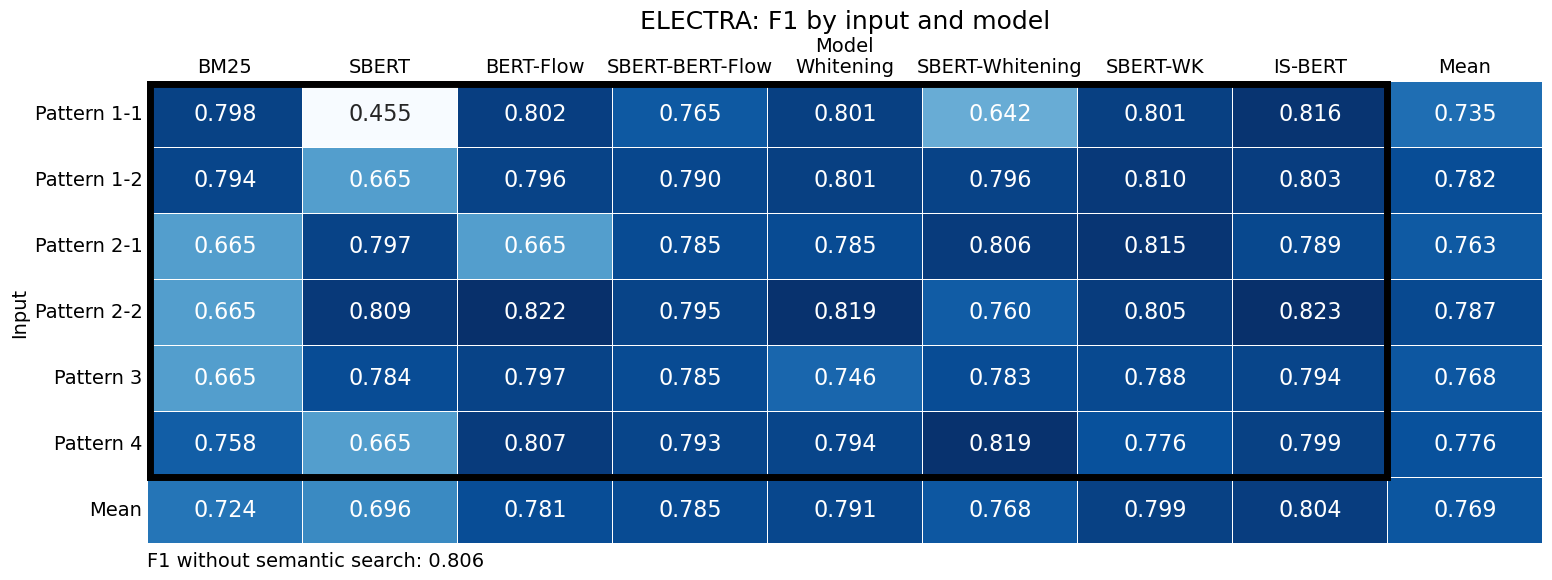
\includegraphics[width = 1\linewidth]{figures/electra_f1.png}
\caption{The F1 score calculated on the test data for all models with ELECTRA as the base model}
\label{fig:electra_f1}
\end{figure}

\begin{figure}[h]
\centering
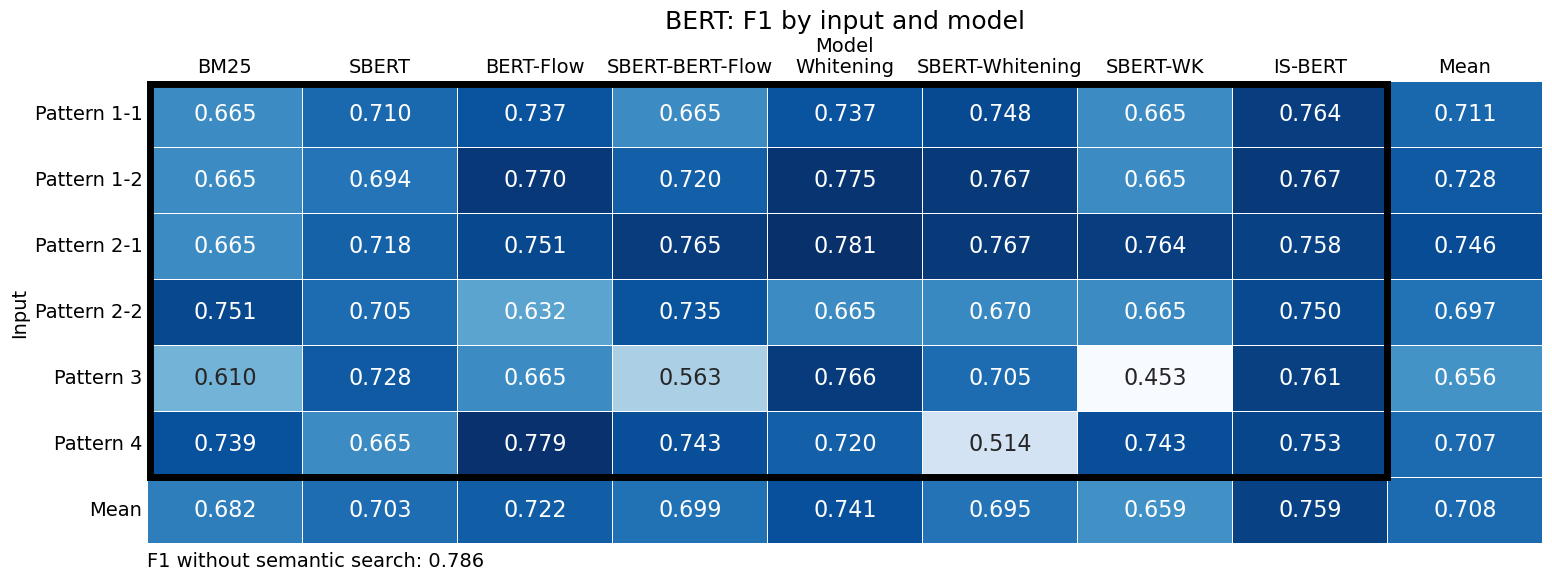
\includegraphics[width = 1\linewidth]{figures/bert_f1.png}
\caption{The F1 score calculated on the test data for all models with BERT as the base model}
\label{fig:bert_f1}
\end{figure}

The results for ELECTRA using the F1 score shown in Figure \ref{fig:electra_f1} mirrored those of the accuracy scores seen in Chapter \ref{results}, with IS-BERT achieving the highest average F1 score of 0.804, while SBERT models gave the worst results. The most effective pattern was Pattern 2-2, whereas the worst-performing pattern was Pattern 1-1.

When looking at the BERT based models in Figure \ref{fig:bert_f1}, the results are also consistent with the accuracy findings. IS-BERT models exhibit the best performance with a mean F1 score of 0.759, while SBERT-WK models perform worse than BM25. Among the input patterns, Pattern 2-1 maintains its position as the best-performing pattern, followed by Pattern 1-2 and Pattern 1-1.

\begin{figure}[h]
\centering
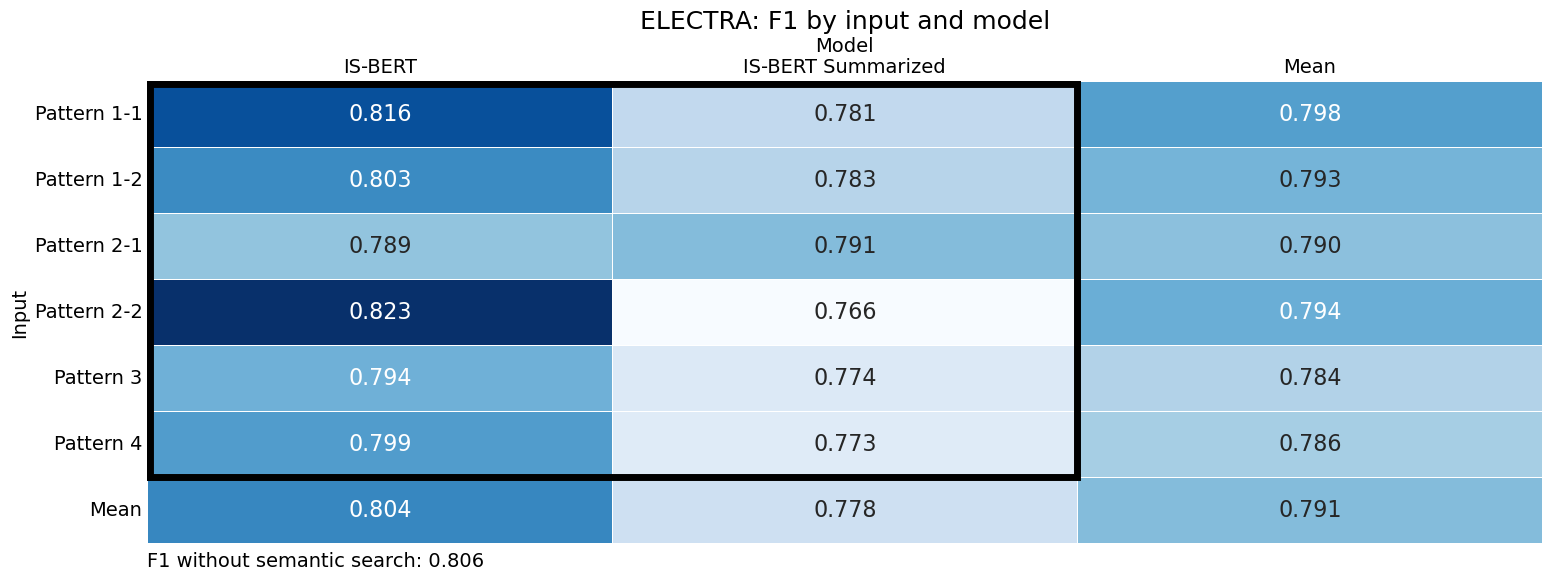
\includegraphics[width = 1\linewidth]{figures/electra_summary_f1.png}
\caption{The F1 score calculated on the test data for the IS-BERT and IS-BERT Summarized models (with ELECTRA as the base model)}
\label{fig:electra_summary_f1}
\end{figure}

The results of Figure \ref{fig:electra_summary_f1}'s F1 score analysis for the summarization experiment support the accuracy's findings. On average, IS-BERT models with summarization perform worse than IS-BERT models without summarization. With an F1 score of 0.791 versus 0.789, the best model (Pattern 2-1) only marginally outperforms the worst IS-BERT model. Other than that, all models perform worse.
